\chapter{B\'{e}zier Intersection Problems}

\section{Intersecting B\'{e}zier Curves}

The problem of intersecting two B\'{e}zier curves is a core building
block for intersecting two B\'{e}zier triangles in \(\mathbf{R}^2\).
Since a curve is a degree one object, the intersections will either
be a curve segment common to both curves (if they coincide) or a finite
set of points.
Many algorithsm have been described in the literature, both
geometric (\cite{Sederberg1986, Sederberg1990, Kim1998}) and
algebraic (\cite{Manocha:CSD-92-698}).

In the implementation for this paper, the B\'{e}zier subdivision
algorithm is used.
In the case of a transversal intersection (i.e. one where the
tangents to each curve are not parallel and both are non-zero),
this algorithm performs very well. However, when curves are tangent,
a large number of (false) candidate intersections are detected and
convergence of Newton's method slows once in a neighborhood of an
actual intersection. Non-transversal intersections
have infinite condition number, but transversal intersections with
very high condition number can also cause convergence problems.

\begin{figure}
  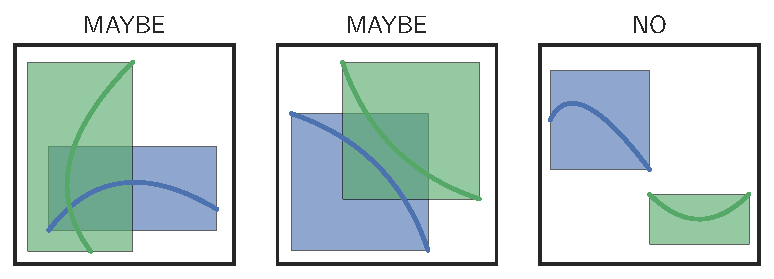
\includegraphics[width=0.9375\textwidth]{../images/curved-mesh/bbox_check.pdf}
  \centering
  \caption{Bounding box check.}
  \label{fig:bounding-box-check}
\end{figure}

In the the B\'{e}zier subdivision algorithm, we first check if the
bounding boxes for the curves are disjoint
(Figure~\ref{fig:bounding-box-check}). We use the bounding boxes
rather than the convex hulls since they are easier to compute and
the intersections of boxes are easier to check.
If they are disjoint, the pair can be rejected. If not, each curve
\(\mathcal{C} = b\left(\left[0, 1\right]\right)\) is split into two halves
by splitting the unit interval \(b\left(\left[0, \frac{1}{2}\right]\right)\)
and \(b\left(\left[\frac{1}{2}, 1\right]\right)\)
(Figure~\ref{fig:bezier-curve-subdivision}). As the subdivision continues,
some pairs of curve segments may be kept around that won't lead to an
intersection (Figure~\ref{fig:bezier-subdivision-process}).
Once the curve segments are close to linear within a given tolerance
(Figure~\ref{fig:bezier-subdivision-linearized}), the process
terminates.

\begin{figure}
  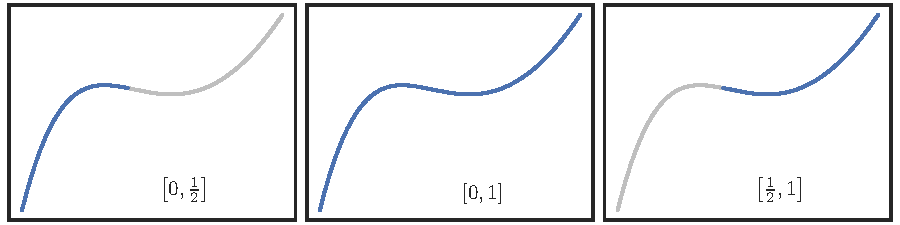
\includegraphics[width=0.9375\textwidth]{../images/curved-mesh/subdivide_curve.pdf}
  \centering
  \caption{B\'{e}zier curve subdivision.}
  \label{fig:bezier-curve-subdivision}
\end{figure}

\begin{figure}
  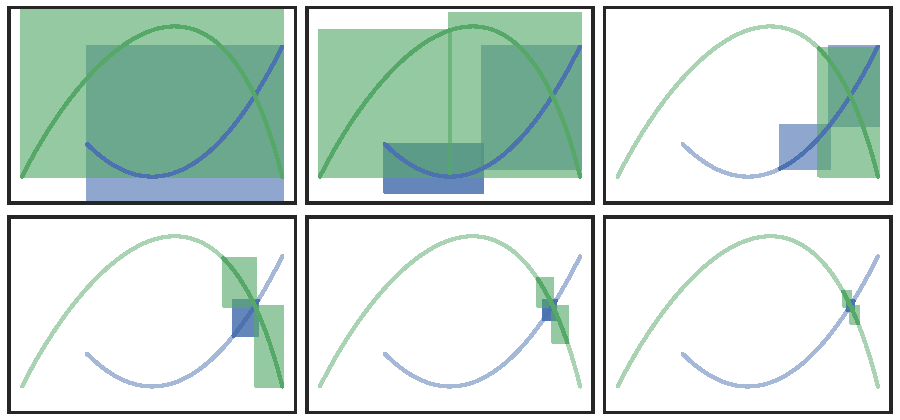
\includegraphics[width=0.9375\textwidth]{../images/curved-mesh/subdivision_process.pdf}
  \centering
  \caption{B\'{e}zier subdivision algorithm.}
  \label{fig:bezier-subdivision-process}
\end{figure}

\begin{figure}
  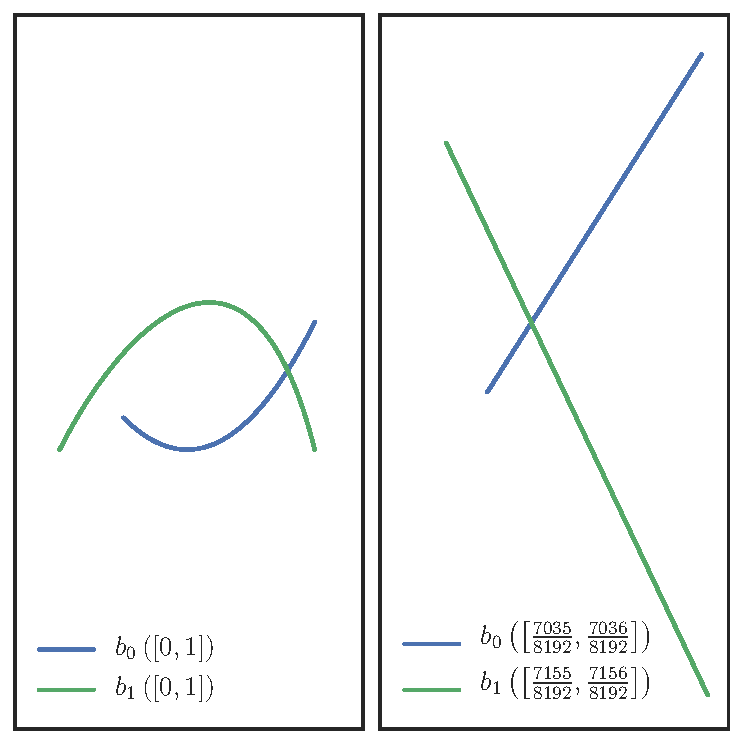
\includegraphics[width=0.96875\textwidth]{../images/curved-mesh/subdivision_linearized.pdf}
  \centering
  \caption{Subdividing until linear within tolerance.}
  \label{fig:bezier-subdivision-linearized}
\end{figure}

\section{Intersecting B\'{e}zier Triangles}

Content.

\section{B\'{e}zier Triangle Inverse}

The problem of determining the parameters \((s, t)\) given a point
\((x, y)\) in a B\'{e}zier triangle...
